% Tiefpass Phasengang (MINIMAL), lineare Achsen, tau = 10 ms
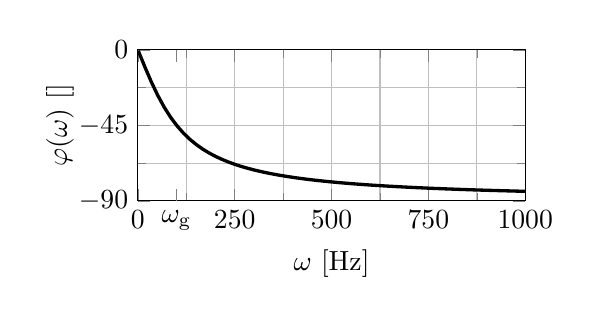
\begin{tikzpicture}[x=1mm,y=1mm] % gilt für tikz-coordinaten außerhalb der axis-environment
    \draw[draw=none] (-14,-12) rectangle (54,22); % Bildrahmen, Koordinatenbezug auf (0,0) des \begin{axis}...\end{axis} pgfplots, für
    \begin{axis}[
        xmode=linear,
        ymode=linear,
        ylabel shift = -5pt,
        ylabel={$\varphi(\omega)\ [\degree]$},
        xlabel={$\omega\ [\mathrm{Hz}]$},
        xmin=0, xmax=1e3,
        domain=1e0:1e3, 
        ymin=-90, ymax=0,
        samples=61,
        width=6.5cm,
        height=3.5cm,
        xtick={0,250,500,750,1000},
        xticklabels={$0$,$250$,$500$,$750$,$1000$},
        ytick={0,-45,-90},
        yticklabels={$0$,$-45$,$-90$},
        minor tick num=1,
        grid=both,
        extra x ticks={100},
        extra x tick labels={$\omega_{\mathrm{g}}$},
        extra tick style={grid=none},
    ]
        %\addplot[mark=none] coordinates{(0,0)} node[anchor=west,black,xshift=5pt] {$\varphi(\omega)\ [\degree]$}; % yaxis label in graph
        %\addplot[mark=none] coordinates{(500,-90)} node[anchor=center,black,yshift=-1pt] {$\omega\ [\mathrm{Hz}]$};      % xaxis label in graph

        \addplot[mark=none,very thick,]   {atan(-x*0.01)}; % 1/(1+(omega*100*100*10^-6)^0.5)^2 % 100 Ohm, 100 uF

    \end{axis}
\end{tikzpicture}